\section{Obstacles in Migrating Concept Erasure to Single-Stream Models}

\label{sec:motivation}
% 0113
\begin{figure}[t]
	\centering
	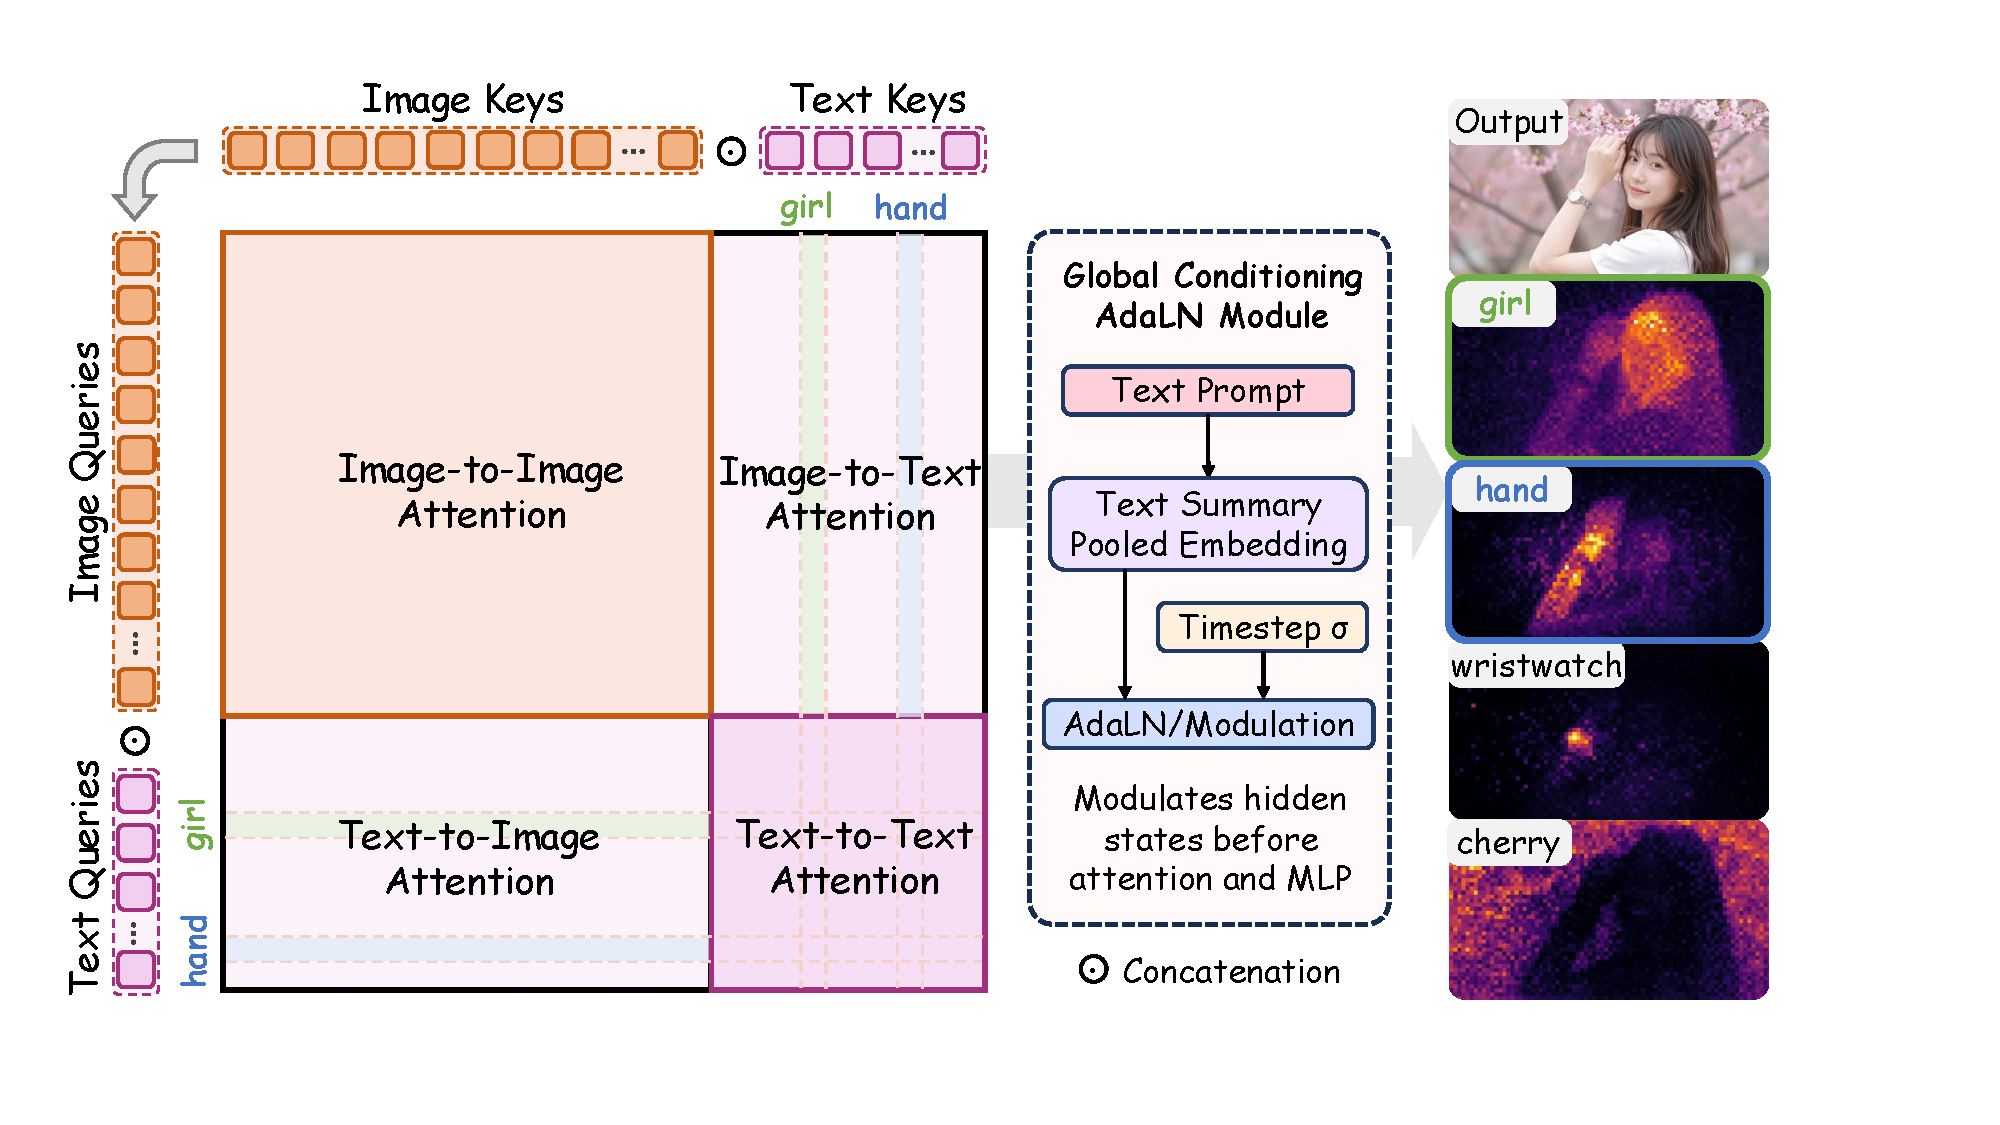
\includegraphics[width=\linewidth]{fig/single_stream_attn.pdf}
    \caption{\textbf{Single-stream attention analysis.} Given the prompt \textit{``A girl with a wristwatch on her hand amid cherry blossoms"}, the attention maps reveal distinct localized responses for text tokens.}
    \label{fig:single_stream_attn}
    \vspace{-10pt}
\end{figure}

% 1223
In this section, we analyze why concept erasure methods designed for SD and dual-stream models (\textit{e.g.}, Flux) fail when applied directly to single-stream architectures. Specifically, we highlight several fundamental obstacles, including the absence of explicit cross-attention mechanisms, the strong coupling between textual and visual representations induced by shared self-attention, and the limited robustness of naive localization-based strategies.

\textbf{Absence of explicit cross-attention:}
The first key challenge is single-stream models like Z-Image lack explicit cross-attention layers (see Appendix~\ref{appendix: Single-Stream Transformer Architecture} for detailed architecture). As a result, methods such as ESD, UCE, and MACE, which originally optimize cross-attention parameters should be redesigned to adapt the new architecture.

This observation naturally raises a question: \emph{Although explicit cross-attention does not exist, does single-stream transformers exhibit a similar pattern between text and image tokens?} Motivated by this possibility, we conduct an in-depth examination of
the neurons and features within the single-stream architecture.



% 0113
\begin{figure}[t]
	\centering
	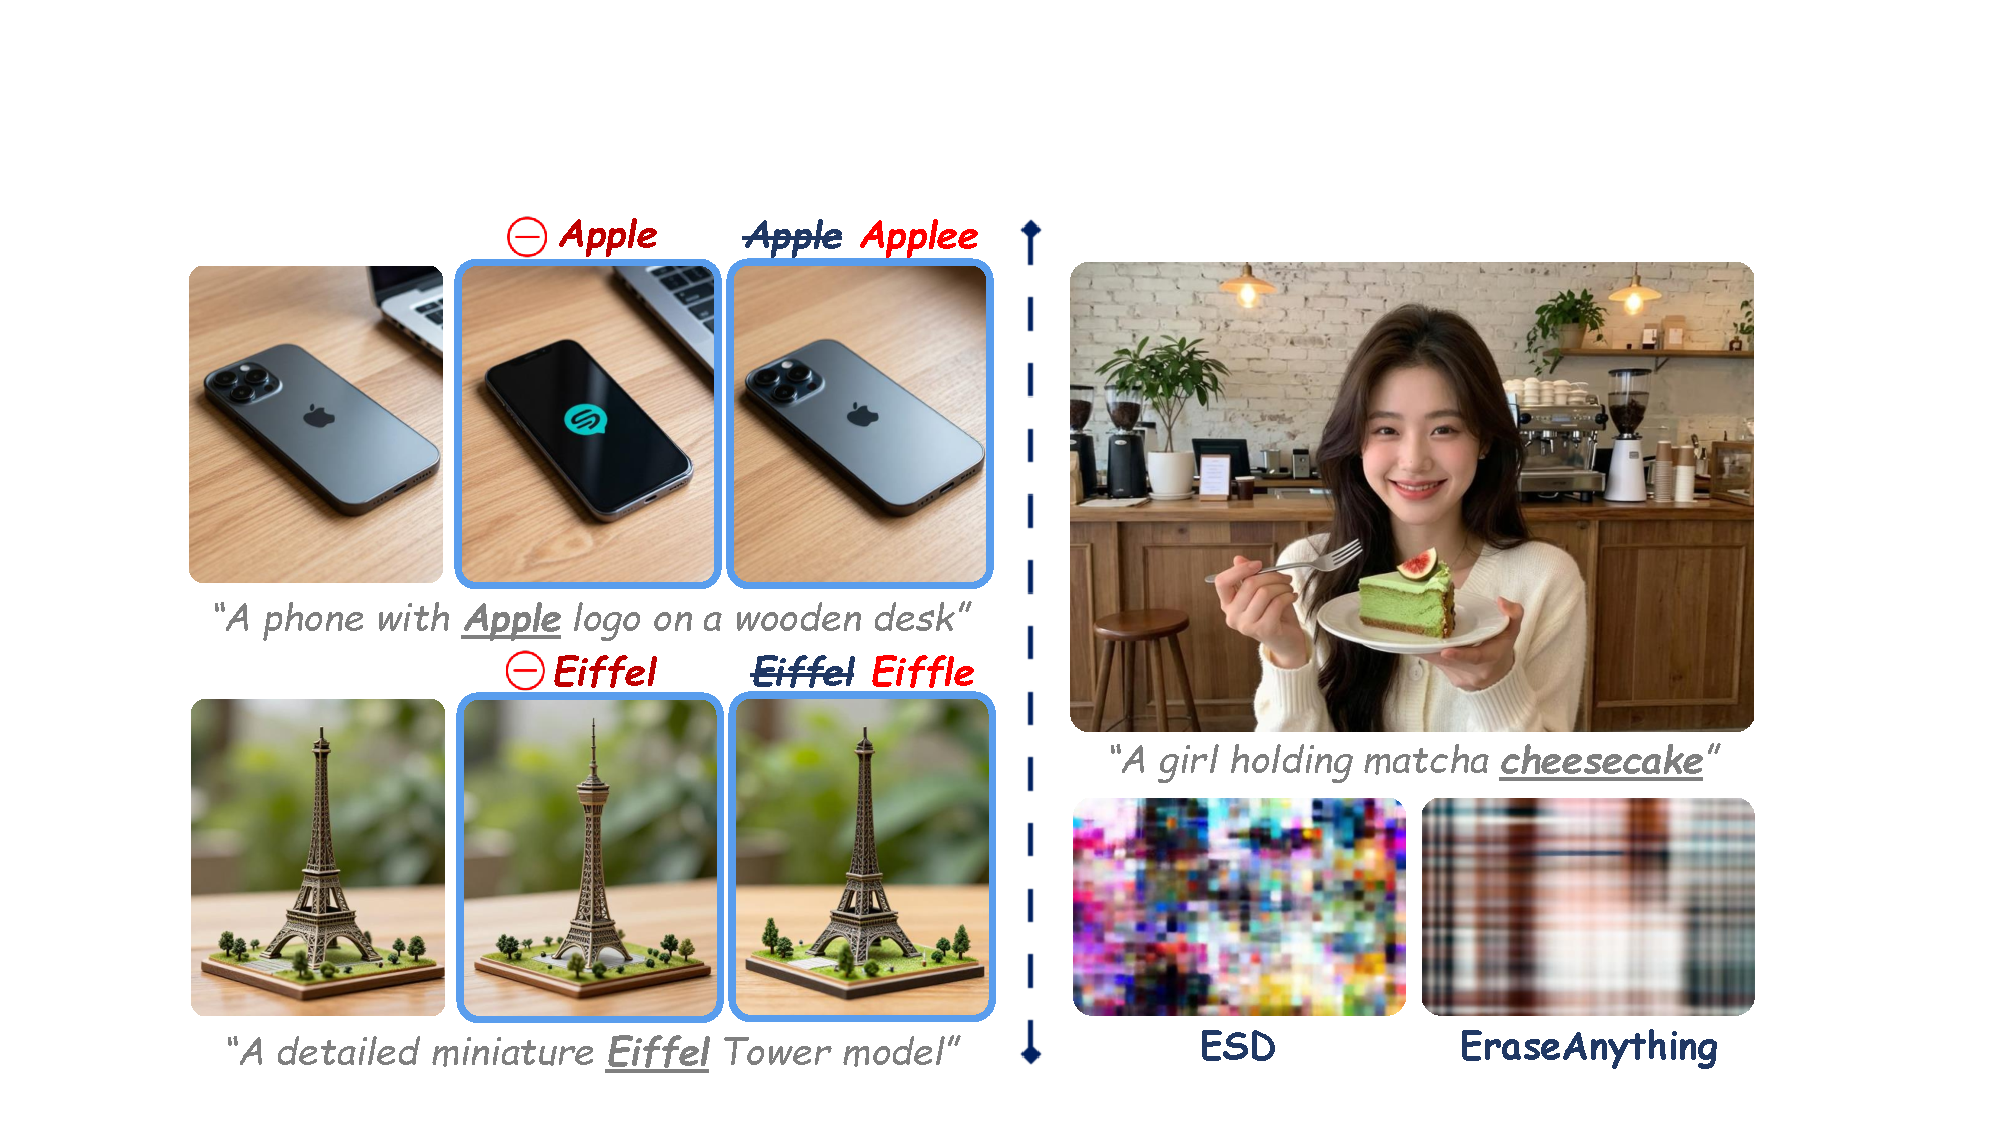
\includegraphics[width=\linewidth]{fig/token_zeroing.pdf}
    \caption{\textit{Left:} \textbf{Attention erasure is brittle.} Concept can be erased by zeroing its attention columns $\mathbf{A}_{attn}[:, :, idx] = 0$ once the target token is localized from the prompt. However, this trick shows poor robustness to real-world prompt variations. \textit{Right:} \textbf{Naive fine-tuning collapses.} Directly fine-tuning shared projections in single-stream models collapses generation with noisy outputs.}
    \label{fig:token_zeroing}
    \vspace{-5pt}
\end{figure}


% dim = 0 删除
\textbf{Single-stream attention:}
We ultimately find that the similar pattern of text–image interactions is encoded through self-attention. Specifically, in modern single-stream models (like Z-Image), visual and textual information are not processed by separate encoders but are instead treated as a single unified sequence. Let $\mathbf{H} \in \mathbb{R}^{(n_I + n_T) \times d}$ denote the input hidden states. The sequence concatenation is defined as:
\begin{equation}
    \mathbf{H} = \mathtt{concat}(\mathbf{H}_{img}, \mathbf{H}_{txt}) \in \mathbb{R}^{(n_I + n_T) \times d},
\end{equation}
where $\mathbf{H}_{img} \in \mathbb{R}^{n_I \times d}$ and $\mathbf{H}_{txt} \in \mathbb{R}^{n_T \times d}$. Unlike dual-stream architectures, which employ separate projection matrices for vision and language,  single-stream models use shared weights $\mathbf{W}_Q, \mathbf{W}_K, \mathbf{W}_V \in \mathbb{R}^{d \times d_k}$ for both modalities. The query, key, and value matrices are computed as:
\begin{equation}
\begin{aligned}
    &\mathbf{Q} = \mathbf{H} \mathbf{W}_Q = \begin{bmatrix} \mathbf{H}_{img}\mathbf{W}_Q \\ \mathbf{H}_{txt}\mathbf{W}_Q \end{bmatrix} = \begin{bmatrix} \mathbf{Q}_{img} \\ \mathbf{Q}_{txt} \end{bmatrix}, \\
    &\mathbf{K} = \mathbf{H} \mathbf{W}_K = \begin{bmatrix} \mathbf{H}_{img}\mathbf{W}_K \\ \mathbf{H}_{txt}\mathbf{W}_K \end{bmatrix} = \begin{bmatrix} \mathbf{K}_{img} \\ \mathbf{K}_{txt} \end{bmatrix}, \\
    &\mathbf{V} = \mathbf{H} \mathbf{W}_V = \begin{bmatrix} \mathbf{H}_{img}\mathbf{W}_V \\ \mathbf{H}_{txt}\mathbf{W}_V \end{bmatrix} = \begin{bmatrix} \mathbf{V}_{img} \\ \mathbf{V}_{txt} \end{bmatrix}.
\end{aligned}
\end{equation}
The self-attention operation $\mathbf{A}_{attn} = \mathtt{Softmax}(\frac{\textbf{Q}\textbf{K}^\top}{\sqrt{d_k}})$ then yields a $2 \times 2$ block matrix representing intra- and inter-modality interactions:
\begin{equation}
\begin{aligned}
    &\mathbf{A}_{attn}
    =
    \mathtt{Softmax}\!\left( \frac{1}{\sqrt{d_k}} 
    \begin{bmatrix}
    \underbrace{\mathbf{Q}_{img}\mathbf{K}_{img}^\top}_{\mathbf{A}_{I \leftarrow I}}
    &
    \underbrace{\mathbf{Q}_{img}\mathbf{K}_{txt}^\top}_{\mathbf{A}_{I \leftarrow T}}
    \\[6pt]
    \underbrace{\mathbf{Q}_{txt}\mathbf{K}_{img}^\top}_{\mathbf{A}_{T \leftarrow I}}
    &
    \underbrace{\mathbf{Q}_{txt}\mathbf{K}_{txt}^\top}_{\mathbf{A}_{T \leftarrow T}}
    \end{bmatrix}\right) .
\end{aligned}
\end{equation}
Here, the cross-terms $\mathbf{A}_{I \leftarrow T}$ and $\mathbf{A}_{T \leftarrow I}$ are intrinsic to the self-attention mechanism, creating \emph{a tight coupling between image generation and text conditioning}, as shown in Fig.~\ref{fig:single_stream_attn}.





% 0113
\textbf{Attention intervention is effective yet brittle:} 
The above analysis suggests that the interaction between text and image is directly formed within $\mathbf{A}_{attn}$: if we locate the target token in the prompt and zero out its attention column, the concept can be removed rather easily. However, this simple trick breaks once the prompt is even slightly altered—adding prefixes/suffixes (\textcolor[rgb]{0.1, 0.2, 0.4}{\textbf{Apple}} $\rightarrow$ \textcolor{red}{\textbf{Applee}}) or intentional misspellings (\textcolor[rgb]{0.1, 0.2, 0.4}{\textbf{Eiffel}} $\rightarrow$ \textcolor{red}{\textbf{Eiffle}}) is enough to bypass the erasure and still generate the concept, as shown in Fig.~\ref{fig:token_zeroing} (left). In other words, \emph{deleting a single attention column is brittle and not robust to real-world prompt variation}, which motivates approaches that modify the model itself through fine-tuning.





\textbf{Naive fine-tuning fails:}
However, we find that directly applying the fine-tuning concept erasure methods such as ESD (for SD v1.5) or EraseAnything (for Flux) on single-stream models consistently causes generation collapse, as shown in Fig.~\ref{fig:token_zeroing} (right). The failure stems from the shared projection weights $\mathbf{W}_Q,\mathbf{W}_K,\mathbf{W}_V$, which jointly serve text conditioning and image synthesis. Therefore, suppressing a textual concept will inevitably perturb the image token pathway through shared self-attention, making controlled concept erasure infeasible. These observations indicate that single-stream models require a dedicated erasure framework that respects this architectural coupling.

